\chapter{Operations at Sea and Field Work in Guaymas Basin}
\label{chap:opsatsea}
%Preface that the intent of this chapter is to highlight practical engineering necessities and opportunities for deep sea research.

\begin{center}
    \begin{minipage}{0.6\textwidth}
      \begin{small}
        How inappropriate to call this planet Earth when it is quite clearly Ocean.\\ \emph{Arthur C. Clarke}
      \end{small}
    \end{minipage}
    \vspace{0.5cm}
\end{center}

Field robotics is a subfield of robotics research devoted to enabling sophisticated robotic autonomy or control in natural environments for performing real\footnote{As in, the task has consequences/stakeholders associated with the performance of the vehicle and the data it collects.} tasks.
This thesis presents autonomy tools for the problem of hydrothermal plume charting in the Guaymas Basin, Gulf of California using AUV \Sentry. 
This chapter provides a description of the Guaymas Basin and the expeditionary cruise in which \Sentry was used for plume charting.
Additional insights on the general challenge of deploying robots for deep sea research, what going to sea entails, and details on operations that complimented the autonomy study are also discussed. 

\section{Guaymas Basin and Expedition RR2107}
\label{sec:guaymas_description}
In November 2021, research cruise RR2107 aboard the research vessel (R/V) \emph{Roger Revelle} was conducted at the Guaymas Basin in the Gulf of California (Mexico).
The Guaymas Basin is located centrally in the Gulf of California, which lies between the Baja peninsula and mainland Mexico (\cref{fig:ops_map}).
The Guaymas Basin is an early rifting environment at a depth of \SI{2000}{\meter}\autocite{scholz2019shelf,moore1982geologic,teske2016guaymas}, meaning that hydrothermal fluids circulate from (geologically) young oceanic crust\footnote{Mainland Mexico and Baja California separate at a rate of approximately 5-\SI{6}{\cm\per\year} \autocite{lonsdale1985hydrothermal}}.
Unlike at mid-ocean ridges, magmatic expressions in the Basin are generally doleritic sill instrusions in thick, organic-rich sediments, rather than extrusive basaltic crusts\autocite{lonsdale1985hydrothermal,teske2019characteristics}.
As these intrusions are often shallow, hydrothermal fluids circulating from the sediments are typically biogeochemically rich; iron\autocite{scholz2019shelf}, methane and carbon dioxide\autocite{geilert2018formation}, and manganese\autocite{campbell1988manganese} have been particularly noted in previous studies.


\begin{figure}[!ht]
  \centering
  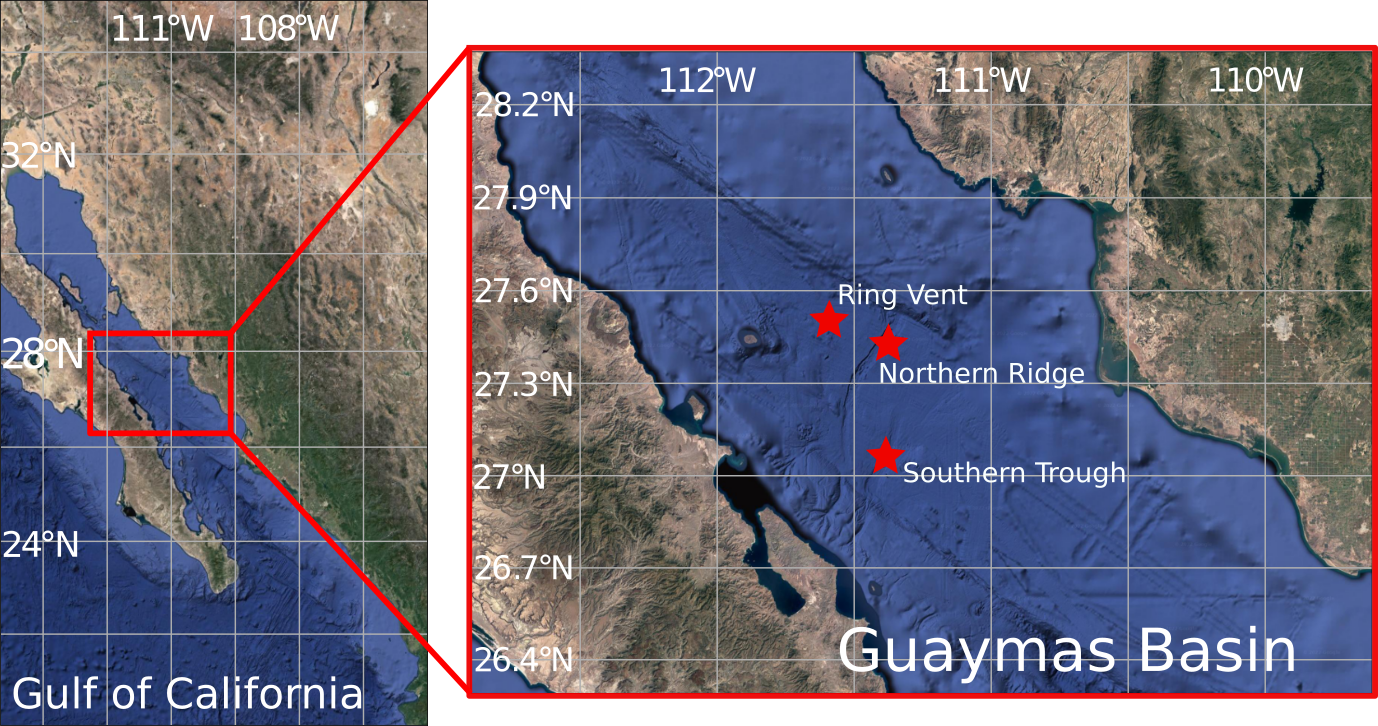
\includegraphics[width=\columnwidth]{figures/ops_guaymas.png}
  \caption[Guaymas Basin, Gulf of California.]{\textbf{Guaymas Basin, Gulf of California.} The Gulf of California and the Guaymas Basin within it are visualized with satellite imagery and composite satellite and open-source bathymetry (as provided by GoogleTiles). The Southern Trough, Northern Ridge, and Ring Vent are marked with stars; the Northern Ridge and Ring Vent were of particular focus during research cruise RR2107.}
  \label{fig:ops_map}
\end{figure}

There are two axial troughs (spreading segments) in the Guaymas Basin, commonly referred to as the Northern and Southern Trough. There has been a long documented history of hydrothermal expressions in the Guaymas Basin, with a particular focus on the Southern Trough\footnote{e.g., \autocite{ondreas2018recent, teske2016guaymas, seewald1994variations, von1985chemistry, lonsdale1985hydrothermal}}. RR2107 was uniquely focused on studying two Northern sites at or near the Northern Trough: Northern Ridge and Ring Vent. Ring Vent is a diffusive off-axis venting site approximately \SI{28}{\kilo\meter} northwest of the Basin spreading center\autocite{teske2019characteristics}. Due to it's nature, ROV \emph{JASON} was primarily used at this site for geochemical surveys. AUV \Sentry studies were instead primarily focused on the Northern Ridge, a recently discovered hydrothermal site\autocite{soule2018exploration, geilert2018formation}, approximately \SI{1850}{\meter} underwater and at the edge of an additionally \SI{300}{\meter} deeper graben. The ridge is approximately \SI{600}{\meter} long and features several tall sulfide structures 10-\SI{25}{\meter} in height with active smoking along their bodies. A smoking ``chimney'' at the northernmost point of the ridge was targeted for autonomous plume-charting, although the entire ridge was studied during RR2107 activities. The chimney vent is composed of a cluster of tens of small orifices ($<$\SI{0.1}{\meter} diameter) that can create up to an approximately \SI{1.5}{\meter} diameter chimney base. The fluid produced is thick with particulate matter and highly-enriched in carbon dioxide, hydrogen, and methane. Measured with a temperature wand on ROV \emph{JASON}, fluid temperature at the vent orifice is estimated to be \SI{340}{\celsius} and the fluid visually ventilates rapidly\footnote{In contrast, the ambient seawater is methane-poor, considerably less turbid, and cold at \SI{4}{\celsius}}. As vent fluids rise and form a plume at this site, the ambient water mixes (entrains) at an unknown rate, and advects by mild deep-water currents estimated to be approximately \SI{0.15}{\meter\per\second} at it's peak during the expedition. Under these conditions, plume expressions could be transported several kilometers from a known source, and would be expected to rise over \SI{200}{\meter} in the water column\autocite{speer1989model}.

The RR2107 expedition had several key objectives: test novel \emph{in situ} instruments to measure dissolved methane\autocite{kapit2021dissolved,kapit2021measurement,michel2022gas}, test novel \emph{in situ} instruments to measure the carbonate cycle, map the heat distribution in shallow sediments above hydrothermal sills\footnote{In extension of, e.g., \autocite{neumann2022heat}}, collect tubeworm and geological specimens, and collect biological samples of microbiota in hydrothermal plume-fluids to re-construct the structure of a plume microbiome. It is typical that research cruises have several science teams working together under an appointed chief scientist to maximize the use of ship assets while at sea, and this cruise was no exception. To enable science operations, AUV \Sentry, ROV \emph{JASON}, and standard oceanographic equipment (i.e., Conductivity-Temperature-Depth (CTD) rosette, Niskin carousel, shipboard acoustics) were available. The deployment of autonomy on the cruise for \Sentry operations was coupled with objectives to test \emph{in situ} instruments and collect microbiota samples. For both of these tasks, charting different regions within a plume is important to test the capabilities of the novel instruments and to collect biological samples from a diversity of plume-conditions.


\section{Challenges for Robots and Autonomy in the Deep Ocean}
\label{sec:ops_challenges}
% No GPS, no satellite, only acoustics, very few observatories, etc.
In the Guaymas Basin setting, or any deep ocean research, there are several unique challenges to deploying robotic platforms in contrast to terrestrial applications. Perhaps the most quintessential of these challenges is the conductive nature of water, and its corresponding attenuation of radio frequencies\autocite{qureshi2016rf}. The natural consequence is that ubiquitous terrestrial technologies leveraged by robots and humans alike, such as global positioning satellites (GPS), imaging satellites, and radio-based wireless communication, are not available for underwater navigation, mapping, or communication. The most common alternative for wireless communication underwater are acoustic waves, which can travel hundreds of kilometers and can be used effectively for ranging (e.g., estimating distance and angle between a source and reflector), but have a significantly reduced data transmission rate\autocite{qureshi2016rf}. Global positioning of an underwater platform is typically done via acoustic ranging with a ship, the ship then having access to GPS to perform an appropriate coordinate transformation for the robot. While accurate, the bit-rate and time-of-flight for information transmission is generally not sufficient for constant localization of a vehicle (let alone also requiring a ship to maintain proximity to a platform, and forgo communicating other types of information), and so many state-of-the-art underwater vehicles use a form of ``dead-reckoning'' to estimate their position with inertial sensors. The use of Doppler velocity loggers (DVL), downward facing acoustic sensors that estimate velocity relative to another object, has improved the overall accuracy of dead-reckoning for near seafloor (within \SI{150}{\meter}) navigation\autocite{stutters2008navigation,liu2022dvl,fong2006evaluation,rigby2006towards}. To us a DVL requires proximity to the seafloor (within tends of meters) in order to provide a ``bottom-lock'' useful for navigation; this further restricts an AUV's navigational freedom.

Beyond navigation and communication, the challenge of working in water necessarily impacts that type of scientific sensing that can also be accomplished. Light, just like radio, is also severely attenuated in water; sunlight typically only penetrates the ocean to about \SI{200}{\meter}, and up to \SI{1000}{\meter} in the best conditions\footnote{Depths between 200-\SI{1000}{\meter} are aptly part of the ocean's ``Twilight Zone''\autocite{martin2020oceans}}. This means that vision based technologies, which have enjoyed significant development in robotics for e.g., autonomous driving tasks, are entirely restricted to either shallow depths or very near seafloor studies, in which light sources carried by a platform might be used\footnote{Of course, navigating in the water column near no other structure is not necessarily a setting for which vision-based navigation may be useful, even if there was light.}. Other common optical-based sensors in robotics, such as Lidar, are similarly difficult to use underwater due to attenuation and refraction. This is not to say that there are no optical sensors that can be used underwater. For short distances, transmitted light between a source and receiver can be used to estimate water turbidity\autocite{bishop1999transmissometer}. Light can also be used to transmit information between a source and a receiver at a higher bitrate than acoustics over modest distances (tens of meters)\autocite{qureshi2016rf,farr2010integrated}. Other sensors may use light, but in creative ways---for instance, oxygen optodes detect luminesence of a chemical reaction that corresponds to a measure of dissolved oxygen\autocite{nicholson2017air}, and laser-based spectrometers have been put in depth-capable housing and use membrane inlets to accept gaseous samples to analyze\autocite{wankel2010new}. While many of these technologies are still in their nascent development phase, perhaps one of the most ubiquitous sensors in oceanography (other than acoustic instruments) is the conductivity-temperature-depth (CTD) probe, which uses induction to measure salinity, resistivity to measure temperature, and a pressure sensor to measure depth\autocite{rudnick2007underway}. With these measurements, computation of density is possible, which is the primary driver of water mass mixing in the ocean. 

No matter the sensor, water-column sensing and mapping in the deep sea relies on collecting point observations and reconstructing fields of interest from these incredibly sparse data.
To address this data sparsity issue, there are several large-scale efforts that contribute to the instrumenting and global understanding of the ocean. Argo, an international network of thousands of small buoyancy-controlled floats which drift in the ocean and take basic \emph{in situ} measurements (e.g., temperature, salinity) of the water column up to \SI{6000}{\meter} in depth is one such example\autocite{roemmich2009argo,jayne2017argo}. With a finer degree of control, small glider networks operated by the e.g., Ocean Observatories Initiative (OOI)\footnote{\url{https://oceanobservatories.org/marine-technologies/gliders/}, \autocite{trowbridge2019ocean}}, offer an opportunity for remote targeting of particular regions or depths to study larger-scale phenomenon. Several highly instrumented ``observatories'', such as Martha's Vineyard Coastal Observatory\autocite{austin2000martha} or the Endurance Array in the Northeast Pacific\autocite{barth2018warm}, also serve an important role for collecting highly temporally resolved data at specific sites. It is certainly the case that there is a lot of ocean data; what has yet to be standardized is how to leverage this data for enabling targeted research studies, particularly with highly capable robotic platforms. Central to this challenge is that despite a wealth of data, the ocean is truly vast; in 10 years of available records from Argo, there are no records of a float in the Guaymas Basin\footnote{As determined via the Euro-Argo data exploration tool, accessed November 20, 2022.}. There are no instrumented arrays in the Gulf of California. And glider or robotics studies conducted there have been part of singular research cruises conducted by disparate research teams, with mixed data discoverability and accessibility. 

While initiatives like the UN Ocean Decade\footnote{\url{https://www.oceandecade.org/}} and the NASA EarthData open science program\footnote{\url{https://www.earthdata.nasa.gov/esds/open-science}} stand to transform the challenge of finding data, practically, oceanographic researchers are prepared to continue to be self-sufficient for any given expedition.
For a roboticist, this requires becoming familiar with prior research at a given site (if available) to contextualize how certain sensors will map to a task at hand, the scientific instruments on a vehicle and their operating principles, and the activities of other science team members to effectively share data within the party. Understanding on all of these axes helps to identify any instrumentation gaps for robotic tasks prior to boarding a vessel (so they can be either rectified by preparing new instrumentation, or the impact mitigated by identifying useful proxies), effectively leverage the expertise of the entire science team to inform missions while underway, and clarifies the design of the post-cruise data products to support science objectives.

\section{The Science Party and Responsibilities}
%Establish how computer scientists fit on a ship.
Before a robot even touches the water, a massive amount of operational overhead is necessary to support deep sea studies. In general, deep ocean research requires using an oceanographic vessel. The R/V \emph{Revelle} is one of several ships in the University-National Oceanographic Laboratory System (UNOLS) network of research ships available through federal support by the United States\footnote{Private research institutions outside of this network, like the Schmidt Ocean Institute, also provide some global-class ships available for deep sea research.}. The R/V \emph{Revelle}, operated by the Scripps Institution of Oceanography at the University of California, San Diego\footnote{\url{https://scripps.ucsd.edu/ships/revelle}}, is a 273 ft vessel constructed in 1996 and completed a mid-life retrofit in 2020. The \emph{Revelle} houses 21 crew and 37 science staff for any expedition. A 4000 sq ft laboratory space dominates one deck of the ship, containing storerooms, a computer lab, a science freezer, and wet lab (among other spaces). The ship is additionally equipped with acoustic surveying equipment, a rosette bay and winch, chemical hoods and storage, dredges, and weather stations in addition to general office equipment. Any additional equipment---AUVs, ROVs, specialized sensing equipment, laboratory equipment, computers---is carried on by the science party.

Captain and crew on a research vessel are responsible for the overall safety of the operations, and are key stakeholders in all operations. Marine technicians are crew members that specialize in the scientific instrumentation and infrastructure on a ship, directly working with the science team to assist with deployments and data curation. The science party itself can be a professionally diverse group of trainees, scientists, and engineers from multiple fields. On RR2107, the science party comprised \Sentry and \emph{JASON} teams (approximately 14 personnel), two teams from Woods Hole Oceanographic Institution (WHOI) comprising engineers, computer scientists, and geochemists (approximately 10 personnel), a team from Harvard University and affiliates in biology, geochemistry, and microgenomics (approximately 4 personnel), and a team from Centro de Investigaci\'on Cient\'ifica y de Educaci\'on Superior de Ensenada (CICESE) comprising geodynamicists (approximately 2 personnel); all teams included graduate students. Everyone on a research vessel not only works together, but must live together for the duration of the expedition. This makes oceanographic research (and any ``expeditionary'' travel) a highly unique working environment\footnote{As late as the 1960s women were barred from working on oceanographic vessels, and this unique working environment can lead to modern inclusivity challenges. Recognition of long-standing challenges to diversity and inclusion in oceanography has inspired new curricula for aspiring chief scientists to design supportive at-sea environments, e.g., \url{https://cobra.pubpub.org/}} in which every member is necessary for making the experience productive and supportive.  

For a field roboticist, being a supportive team member may mean performing more than just \Sentry or \emph{JASON} operations. Literacy in certain data processing and visualization tools, comfort with network protocols and a command line, and hands-on experience working with certain sensors can prove to be extremely useful to other science activities while aboard. Coordinating with other science teams prior to an expedition can be a way to identify areas in which a computer scientist or a roboticist could be helpful. For instance, prior to RR2107, a desire to monitor \Sentry science data while it was underway was expressed. While outside of the direct purview of the autonomy operations, creating a tool that listened to a local network on the ship and displaying data that came over the network in a live visualizer was a relatively straightforward process and provided the science team with a ``real-time'' view of \Sentry operations, informative for other activities. In practice, a field roboticist has a lot of tools that they bring with them on an expedition; there is increasing interest in using more of those tools for oceanographic missions as data infrastructure and use of \emph{in situ} sensors accelerates.  

\section{AUV \Sentry}
AUV \Sentry, operated by the National Deep Submergence Facility (NDSF) at WHOI\autocite{kaiser2016design} is a general purpose platform with depth capability up to \SI{6000}{\meter} (\cref{fig:ops_sentry}). \Sentry is the successor of \emph{ABE}\autocite{yoerger1991autonomous}, the first widely utilized AUV for deep ocean research by the U.S. oceanographic community. \Sentry has completed upwards of 600 dives, and is equipped with three classes of instruments: vehicle sensors, geophysical sensors, and oceanographic sensors. Vehicle sensors are largely those that assist with AUV localization; geophysical sensors include acoustic multibeam, subbottom profiler, and magnetometers, which are useful for collecting bathymetric and sub-seafloor maps. For plume studies, the oceanographic sensors are of primary interest, and include a CTD, optical backscatter (OBS) instrument, oxygen optode, and oxidation reduction-potential (ORP) sensor. Each oceanographic sensor is synced to a shared precision clock on \Sentry, and logged to separate files at the manufacturer recommended sampling frequencies. In addition to the standard sensor suites, \Sentry can accept some novel instrumentation developed by a science party for an expedition. During RR2107, two novel methane sensors were integrated into \Sentry to complement the oceanographic sensors for hydrothermal plume charting\autocite{michel2022gas,kapit2021dissolved,kapit2021measurement}.

\begin{figure}[h!]
  \centering
  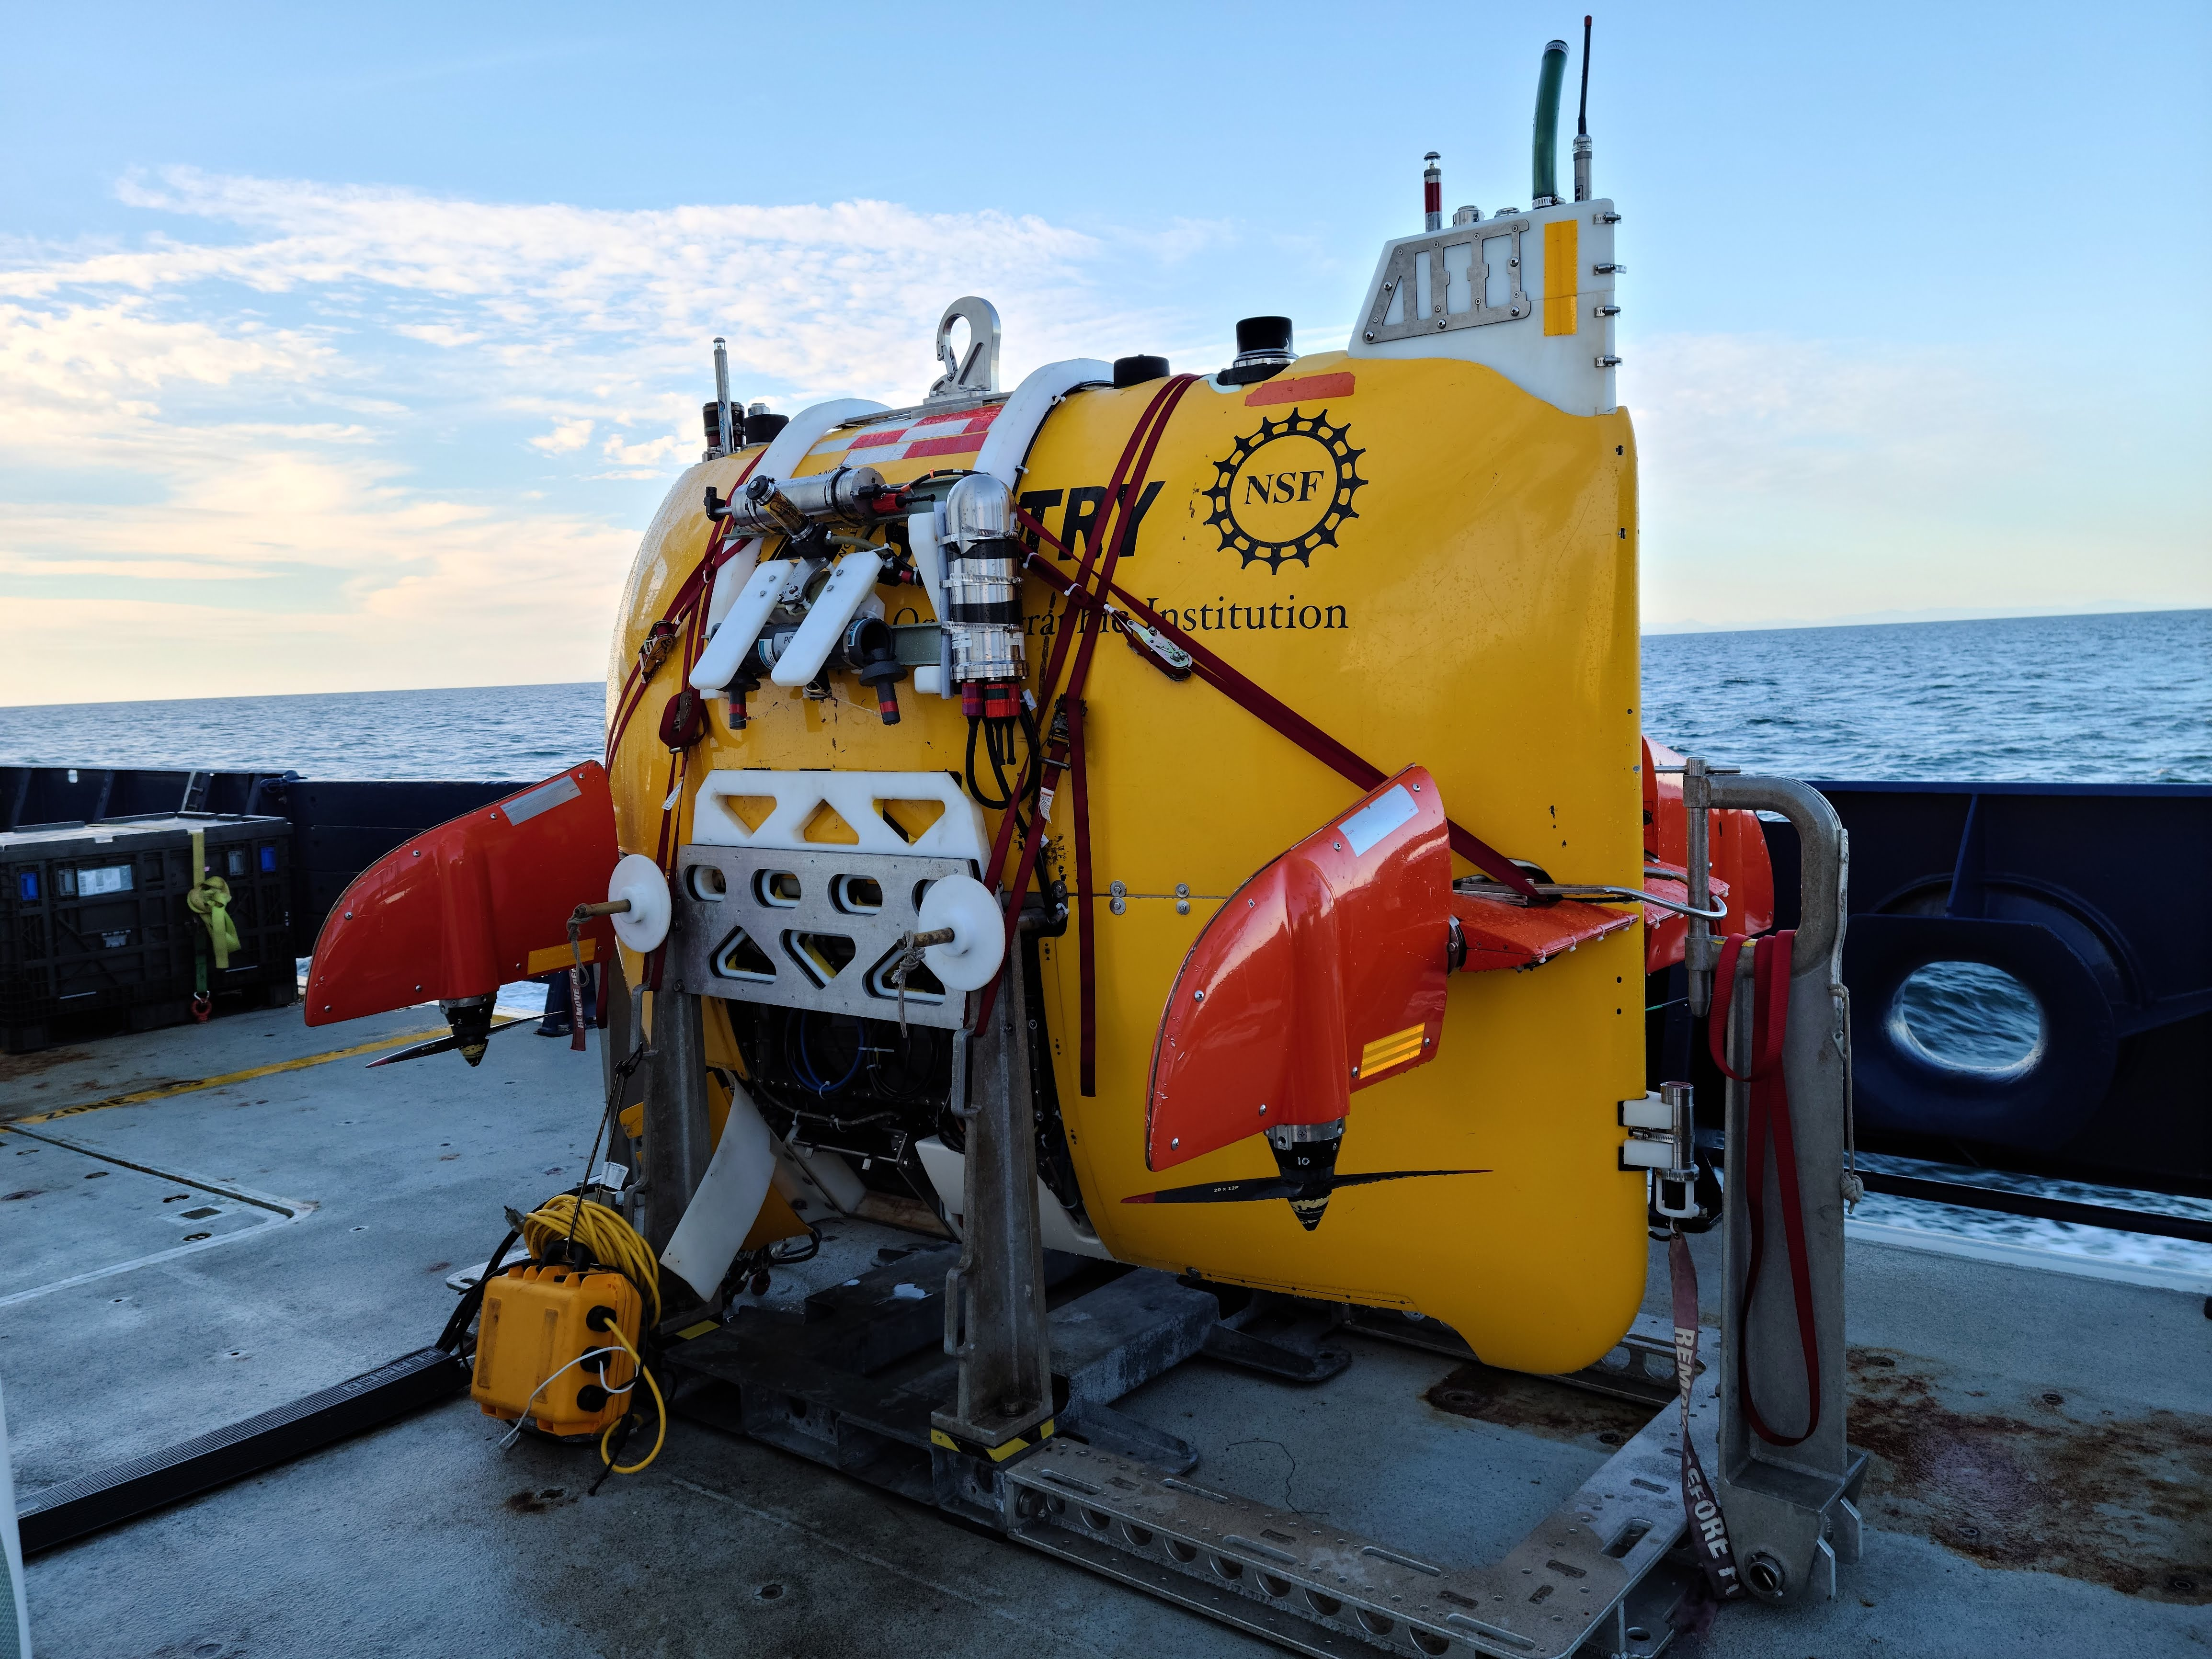
\includegraphics[width=0.8\columnwidth]{figures/ops_sentry.jpg}
  \caption[AUV \Sentry]{\textbf{AUV \Sentry}. A picture of AUV \Sentry on deck of the R/V \emph{Revelle} during RR2107 activities.}
  \label{fig:ops_sentry}
\end{figure}

The \Sentry team for an expedition has an appointed expedition leader, who interfaces directly with the Chief Scientist and any other relevant science parties to plan \Sentry dives. The team is largely responsible for the physical and virtual safety and maintenance of \Sentry during an expedition. As such, the expedition leader is additionally responsible for confirming the safety of every dive plan and managing pre-dive and post-dive checks. Safety confirmation of a dive plan formally requires passing a simulation dive of the plan using a set of scripts maintained by the \Sentry team. This simulation uses bathymetry and marginal environmental estimates to assist in checking a plan for obstacle clearance, in addition to computing possible localization drift (associated with number of turns) among other heuristics. Less formally, the expedition leader has final call on whether a dive is feasible, and may use contextual knowledge of a location or the vehicle state to deny or suggest changes to a plan. For instance, Guaymas Basin has a notably soft seafloor due to sediment deposition. This impacts the quality of DVL estimates, which in turn impacts the quality of \Sentry localization. This lead to adjusting the altitude restriction for \Sentry during RR2107 to reduce risk to the vehicle.


\section{ROV \emph{JASON}}
ROV \emph{JASON}, like AUV \Sentry, is also operated by the NDSF at WHOI\autocite{ballard1993medea,yoerger1986jason,petitt2004power} and has been in operation since the late 1980s (\cref{fig:ops_jason}). Distinct from \Sentry, \emph{JASON} is connected to a ship via a cable which transmits information and power. This allows real-time sensor and visual feedback from the ROV and fine remote control of the vehicle navigation and two manipulator arms. \emph{JASON} is a particularly powerful tool, as it can literally ``put eyes'' on the seafloor, and perform physical sample collection tasks that AUVs cannot, including sediment coring, microbial mat retrieval, macro-flora/fauna and rock sample collection, and water sampling. Standard oceanographic equipment, like CTD, optode, and turbidity sensor are mounted to \emph{JASON} and logged in a similar fashion to \Sentry equipment. \emph{JASON} can additionally accommodate carrying novel equipment brought by a science party, however this equipment must be certified before integration on \emph{JASON} for the desired depth they are to be deployed. 

\begin{figure}[h!]
  \centering
  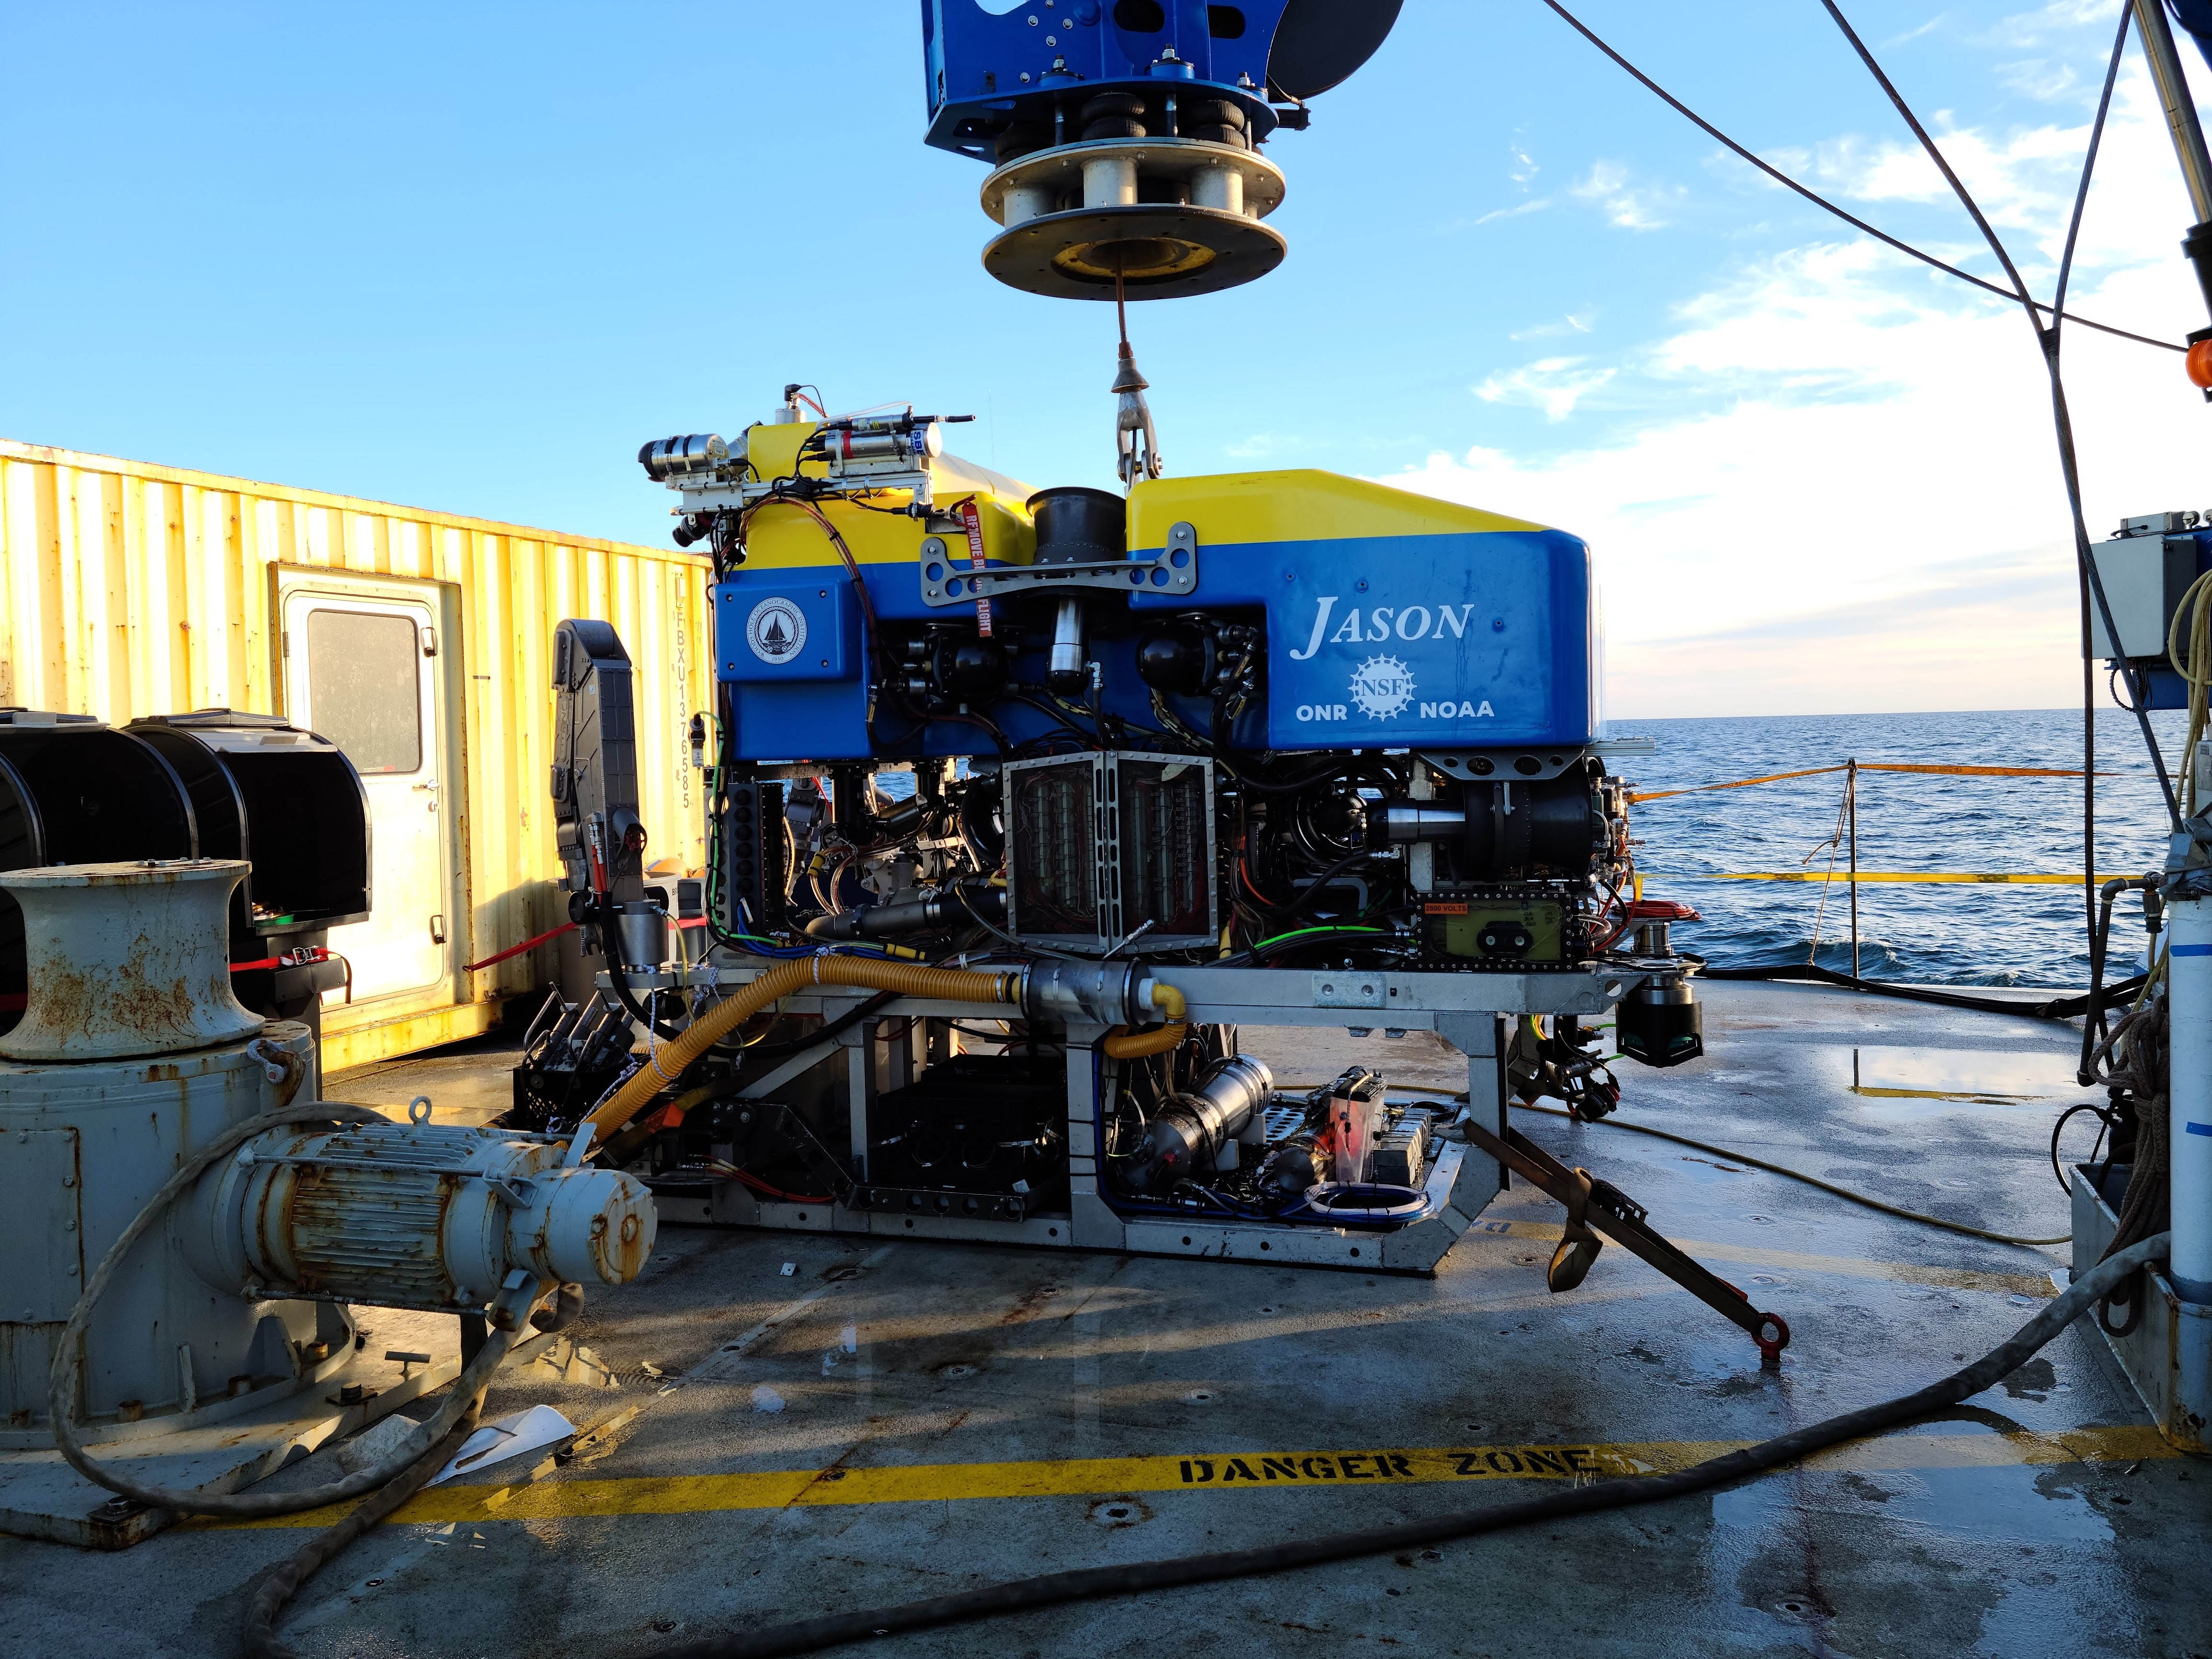
\includegraphics[width=0.8\columnwidth]{figures/ops_jason.jpg}
  \caption[ROV \emph{JASON}]{\textbf{ROV \emph{JASON}}. A picture of ROV \emph{JASON} on deck of the R/V \emph{Revelle} during RR2107 activities.}
  \label{fig:ops_jason}
\end{figure}

While being operated, three \emph{JASON} engineers act as ``pilots'' in rotating shifts throughout a dive (which can be over 24 hrs long). These piloting operations occur in the ``control van'', in which data servers/ship-side data loggers, computer monitors, and annotation stations are set-up. At least three science party members are also required in the control van during operations---a dive science leader and two annotators. The science leader interacts with the pilots and sets the activities for a dive (e.g., collect this rock, collect some video, navigate to a new location). The annotators listen to the science leader and pilots to keep a running log of science activities and any relevant information about a dive as it occurs. The annotated logs are used post-expedition to search through \emph{JASON} data. The science party is responsible for setting a schedule for dive science leaders and annotators. On RR2107, most members of the science party were assigned at least one 4 hour shift in a 24 hour period in which they would be on call for being in the control van if operations were underway.

\paragraph{Autonomy Study Activities}
ROV \emph{JASON} was a rich source of external data to assist with the autonomy study presented in this thesis. In particular, \emph{JASON} could physically observe the target vent and deploy additional sensing equipment to compensate for holes in \Sentry sensing capabilities for the expedition. As described briefly in \cref{chap:field_results}, \emph{JASON} was used to:
\begin{itemize}
  \item Estimate the fluid temperature at a vent orifice with the temperature wand; measured \SI{340}{\celsius}.
  \item Estimate the size of a chimney and vent via still imagery.
  \item Deploy MISO cameras at a vent site, used to estimate the fluid exit velocity at a vent via video.
  \item Deploy current tiltmeters at various locations on the seabed to estimate deep currents at the autonomy test site.
\end{itemize}

While the first two activities are standard for \emph{JASON} studies, the latter two were specific to the operations in RR2107. 
MISO cameras, self-contained depth-capable GoPro devices\footnote{\url{https://www2.whoi.edu/site/miso/}}, were mounted to the brow and one of the arms on \emph{JASON}. Set to record in 4k, the arm-mounted camera was aligned to be approximately parallel with an active vent and used to record 1-5 min videos of turbulent plume fluids. The video was then processed following a \emph{JASON} recovery using particle imaging velocimetry (PIV)\autocite{zhang2019time}, which tracks turbulent ``parcels'' that have high cross-correlation between frames. By tracking many specific parcels over several frames, PIV methods can provide a vector field of velocity estimates, that can then be averaged to provide an estimate of mean flow in a region. Using MatLab's open source \verb|PIVLab|, a representative vent in the basin recorded during \emph{JASON} dive JD1390 at (27.4018606 N, 111.3991182 W, \SI{1809}{\meter} depth) was estimated to have fluid exiting at 0.7-\SI{1.33}{\meter\per\second} (\cref{fig:ops_miso}).

\begin{figure}[h!]
  \centering
  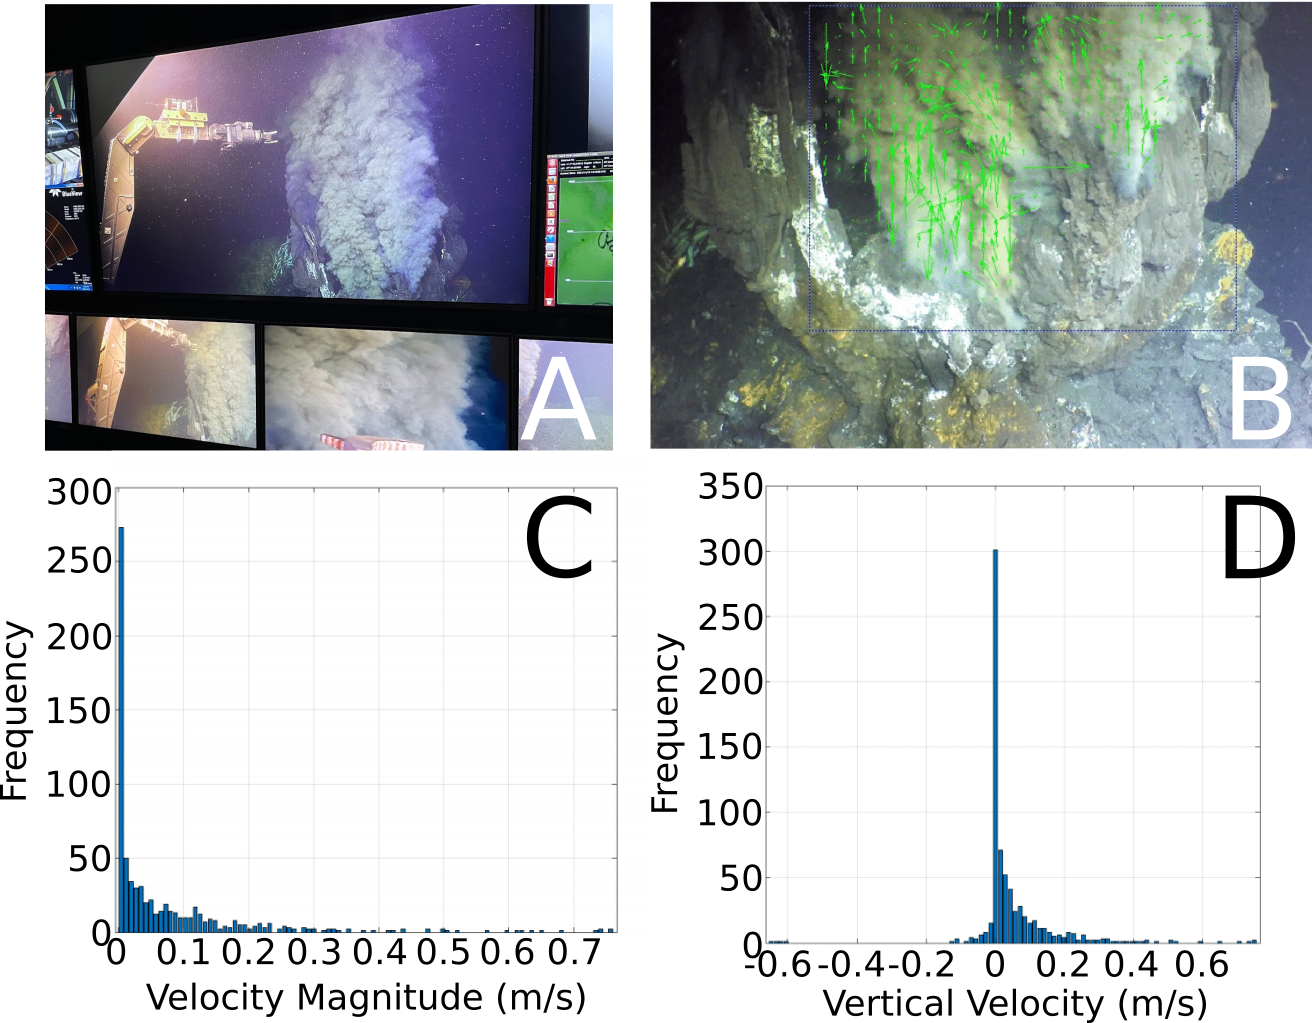
\includegraphics[width=0.8\columnwidth]{figures/ops_miso.png}
  \caption[Exit velocity estimation with WHOI-MISO cameras]{\textbf{Exit velocity estimation with WHOI-MISO cameras.}. A WHOI-MISO camera was mounted on an ROV \emph{JASON} arm and positioned to film exiting plume fluids from a hydrothermal vent (A). The capture video was processed using a PIV technique (B-D), which provides estimates of fluid velocity. The tails of the velocity field distributions may be indicative of exit velocities near orifices, as most of the imaged field is dominated by turbulent mixing within a meter of the orifices.}
  \label{fig:ops_miso}
\end{figure}

Tilt current meters\footnote{\url{https://lowellinstruments.com/}} are mounted to the seafloor by one point and are free to move under crossflow. The pose of the tiltmeter can be directly converted to crossflow magnitude and heading. ROV \emph{JASON} was used to alternately deploy 2 TCM-3 tiltmeters while performing other operations. \cref{tab:ops_tilt} shows information for each deployment. The first deployment of Tiltmeter A was the primary dataset used to generate an estimate of the current function used for the autonomy study. 

\begin{table}[h!]
  \centering
  \begin{tabular}{c|c|c|p{0.3\linewidth}}
      Tiltmeter & Dive Deployed/Recovered & Duration & Location \\
      \hline
      A & JD1389/-- & 28* hrs & (27.4006177 N, 111.3985321 W, \SI{1832}{\meter}) \\
      A & --/JD1390 & 28* hrs & (27.4002362 N, 111.3962494 W, \SI{1854}{\meter}) \\
      B & JD1389/JD1396 & 6 days, 15 hrs & (27.4006177 N, 111.3985321 W, \SI{1832}{\meter}) \\
      A & JD1392/JD1392 & 10 hrs & (27.4149571 N, 111.3873036 W, \SI{1840}{\meter}) \\
      A & JD1393/JD1393 & 20 hrs & (27.5001163 N, 111.6832265 W, \SI{1732}{\meter}) \\
  \end{tabular}
  \caption[Summary of tiltmeter deployments]{\textbf{Summary of tiltmeter deployments.} Two tiltmeters were deployed using ROV \emph{JASON} during RR2107 to estimate the magnitude and heading of deep currents. One tiltmeter was deployed for nearly 1 week, while another was deployed intermittently, so data products self-logged on the instrument could be used for autonomy ops. During the first deployment of tiltmeter A, the tiltmeter was moved to better align logistically with other \emph{JASON} operations.}
  \label{tab:ops_tilt}
\end{table}


\section{CTD Rosette}
A CTD rosette (or just rosette, \cref{fig:ops_rosette}), is a standard piece of oceanographic equipment which is typically an instrumented metal cage connected to a ship via a cable and used to collected vertical transects of the water column. Rosettes can also be towed laterally the water column if lowered and the ship driven in the pattern of the desired transect. Over the cable, data from the instrumentation on a rosette is streamed to a computer terminal on the ship. The depth is controlled by pulling in or releasing cable using a winch. The typical workflow is that one or more science team members are responsible for ``standing watch'' while a rosette is in operation, and communicates to a winch operator (always a crew member) via phone with requests to let out or pull in the cable.

\begin{figure}[h!]
  \centering
  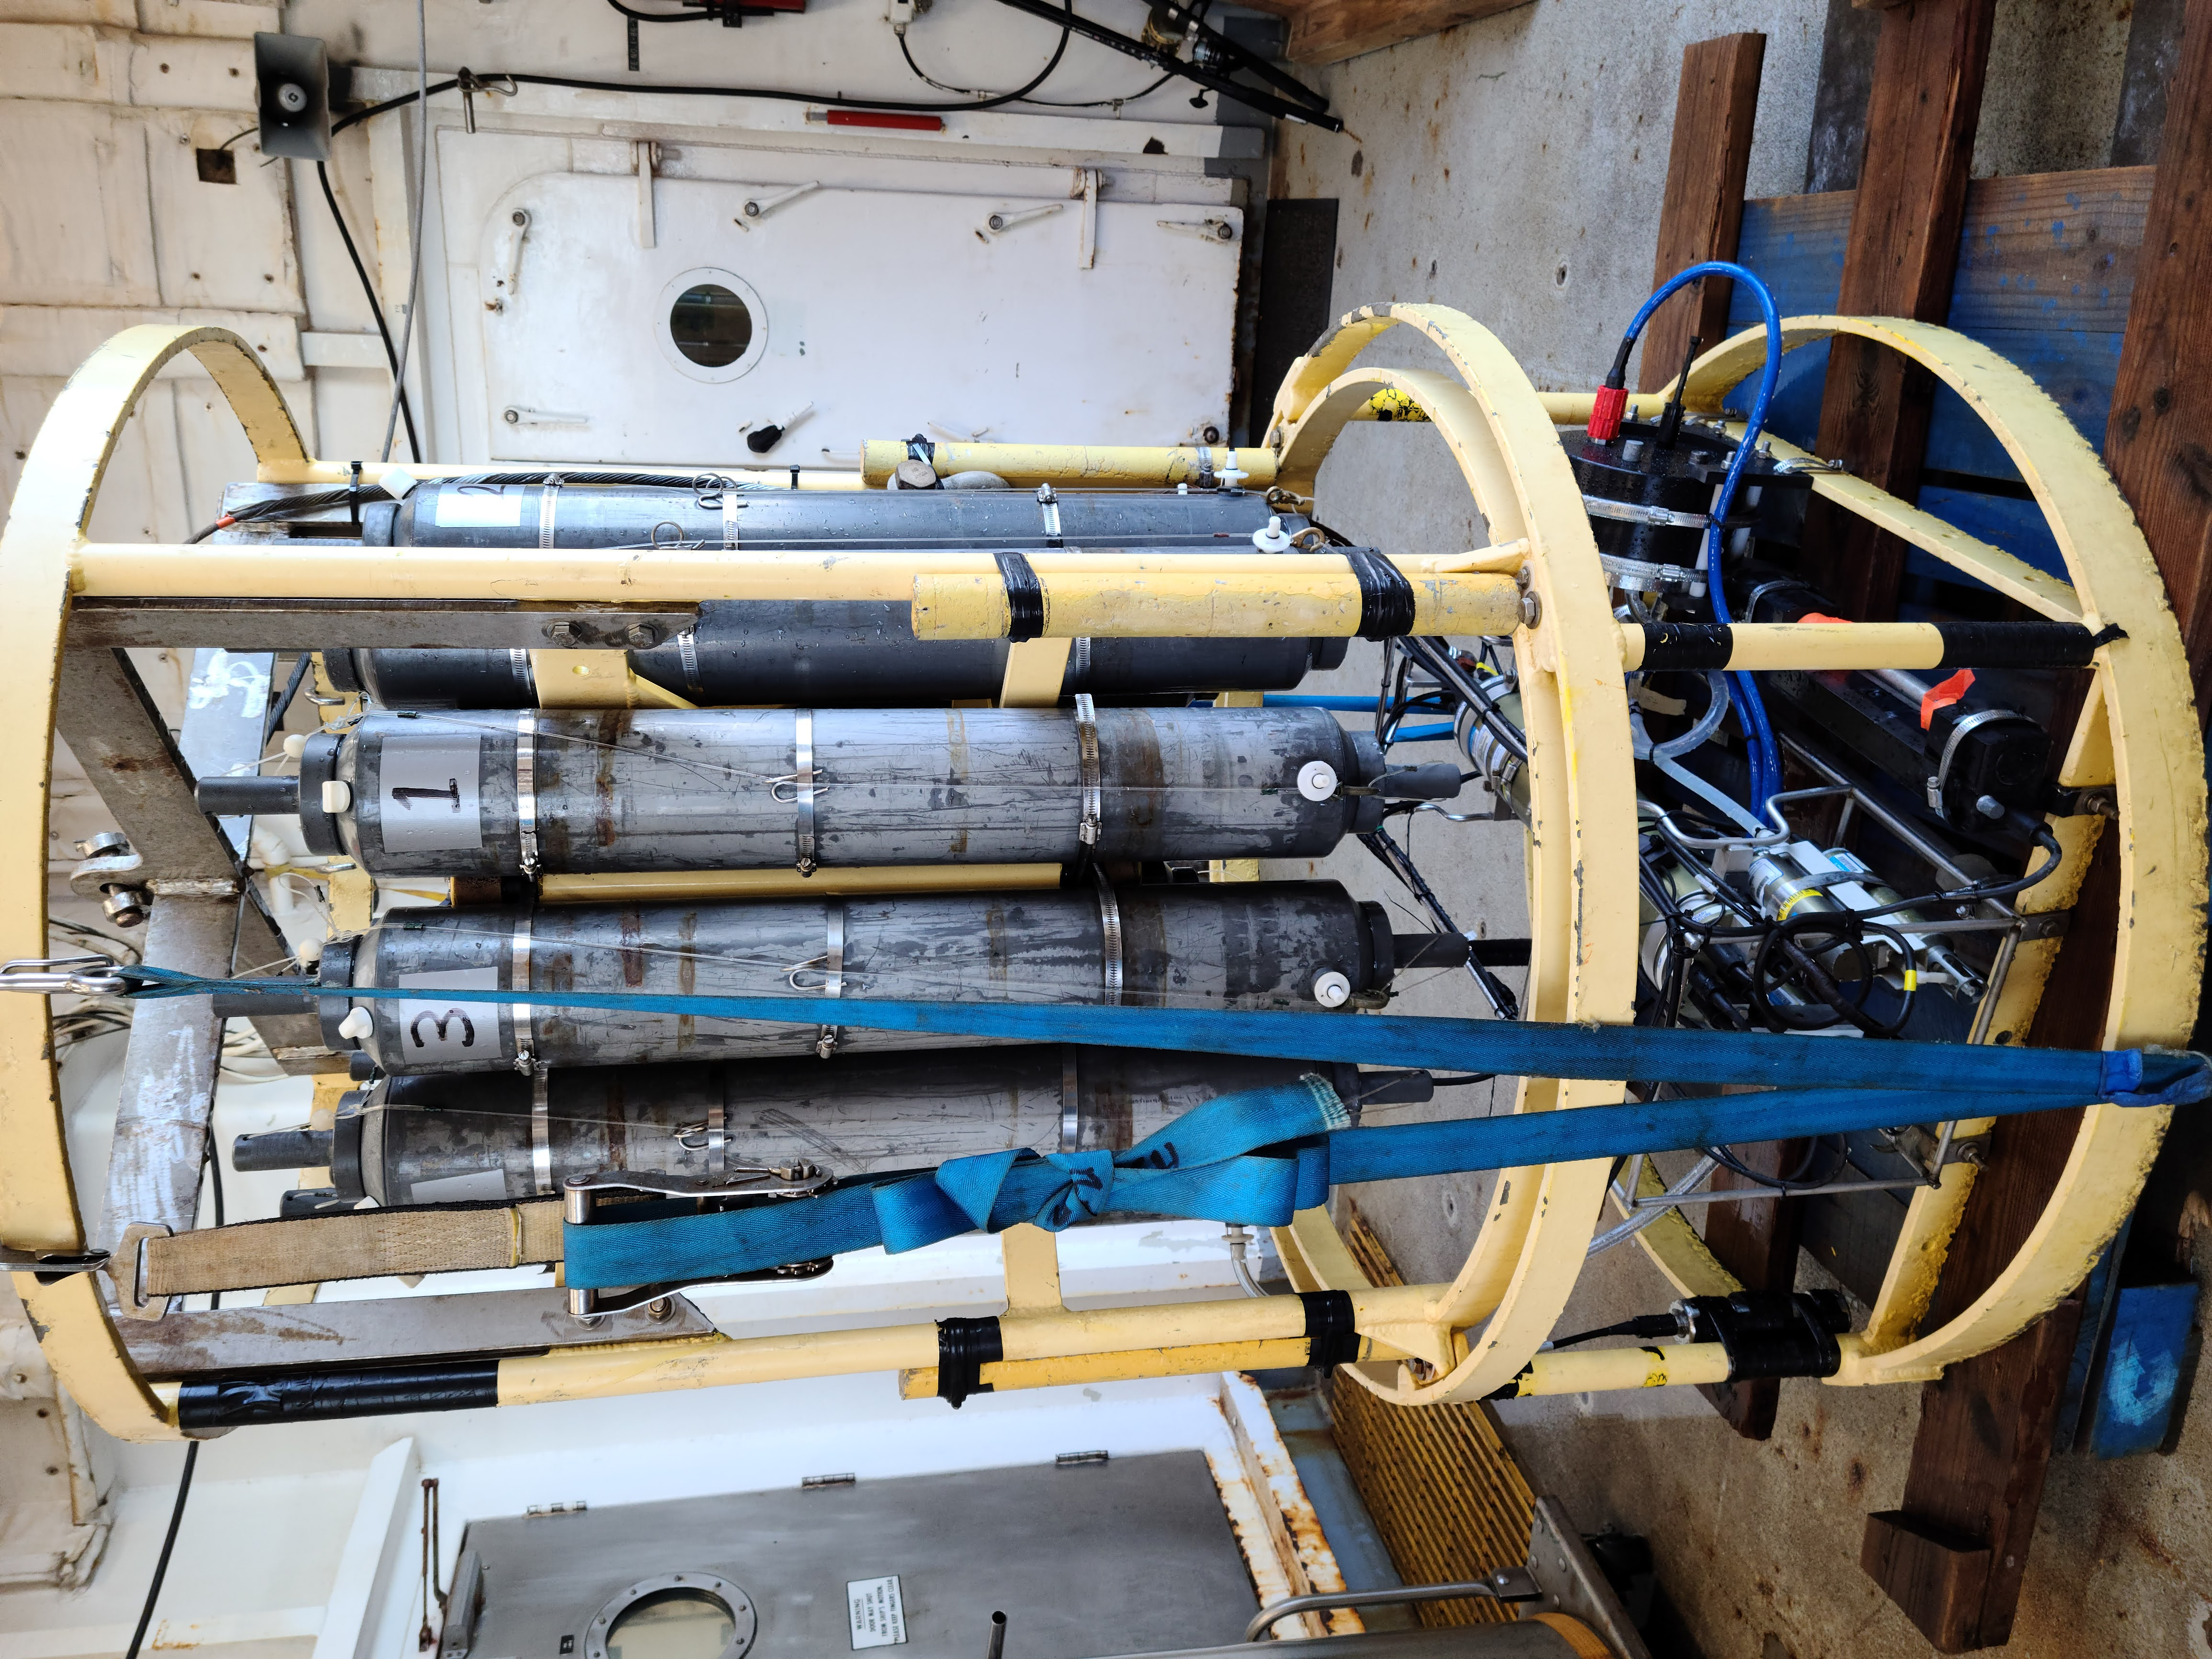
\includegraphics[width=0.8\columnwidth]{figures/ops_rosette.jpg}
  \caption[CTD Rosette]{\textbf{CTD Rosette}. A picture of the rosette in the rosette bay on R/V \emph{Revelle} during RR2107 activities.}
  \label{fig:ops_rosette}
\end{figure}


Equipment available on the rosette for RR2107 included CTD, flourometer, oxygen optode, and transmissometer (turbidity). All data is logged via a shared clock and in a proprietary format by Sea-Bird Scientific\footnote{\url{https://www.seabird.com}}, which was converted to CSV files while aboard the \emph{Revelle}. The rosette also had a 13-bottle Niskin bottle carousel. Niskin bottles are water containers which can be closed (``fired'') to seal water samples for \emph{ex situ} analysis. During rosette operations, Niskin bottles can be closed from the science team computer station by either pre-programming depths before a vertical transect, or by requesting a bottle fire via the monitoring application of the rosette while it is underway. Bottle samples during RR2107 were used to collect microbial samples, dissolved gas samples, and calibrate other \emph{in situ} instrumentation. 11 casts of the rosette were performed, 9 of which were standard vertical profiles. 

\paragraph{Autonomy Study Activities}
Within an analytical model for plume rise, density differences are computed in order to estimate buoyant force, which ultimately drives the estimated neutrally-buoyant layer height.
While standard stratification (density) profiles for the Atlantic and Pacific ocean basins are widely accepted\autocite{speer1989model}, the Guaymas Basin is a unique semi-closed system in the Gulf of California, and a stratification curve for background seawater in this Basin would lend itself to more accurate estimates of plume characteristics. As an AUV descends, it performs a vertical transect that could be used to compute this local stratification curve, however, since in RR2107 operations AUV \Sentry was typically targeted plume-impacted sites, and did not travel lower than an altitude of \SI{30}{\meter} for any operations, using profiles from the rosette would be advantageous. Using a set of subsampled points from every vertical transect collected by the rosette, a Gaussian Process (GP) was fit to the data, and the mean function used as the stratification curve used for autonomy tests.

